% software flow chart
% -------------------

\documentclass[border=0mm,tikz]{standalone}
\usepackage[utf8]{inputenc}
\usepackage{times}
\usetikzlibrary{positioning}
\usetikzlibrary{chains}

\tikzstyle{block} = [rectangle, draw, rounded corners,
                     text width=10em, text centered, minimum height=4em]
\tikzstyle{data}=[block, fill=red!20]
\tikzstyle{soft}=[block, fill=green!20]
\tikzstyle{pism}=[block, fill=blue!20]

\newcommand{\data}[4][]{\node [data, #1] (#2) {\textbf{#3} #4};}
\newcommand{\soft}[4][]{\node [soft, #1] (#2) {\textbf{#3} #4};}

% fancier using shapes.multipart library
%\newcommand{\soft}[4]{\node [draw, rectangle split, rectangle split parts=2,
%                             %rectangle split part fill={blue!50,white},
%                             rounded corners, #1] (#2)
%                             {\textbf{#3}\nodepart{two} #4};}

%  \tikzstyle{data}=[rectangle, minimum size=1cm, draw]
%  \tikzstyle{soft}=[circle, minimum size=2cm, draw]
%  \tikzstyle{pism}=[rectangle, minimum size=2cm, draw]

\begin{document}
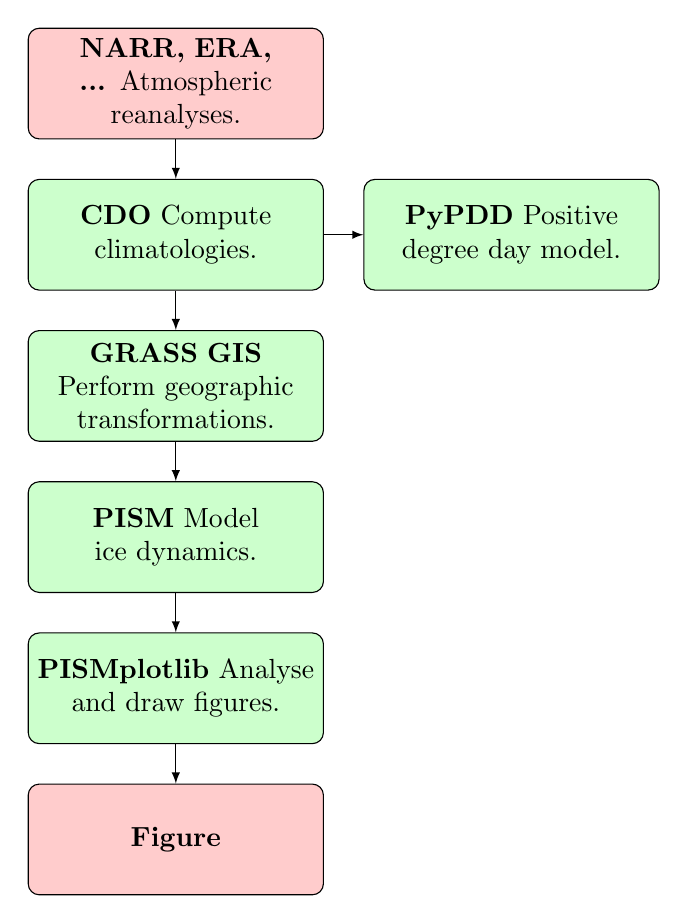
\begin{tikzpicture}[node distance=5mm, start chain=1 going below,
                    every node/.style={on chain, join},
                    every join/.style={-latex}]
  \data {atm} {NARR, ERA, ...} {Atmospheric reanalyses.};
  \soft {cdo} {CDO}
    {Compute climatologies.}
  \begin{scope}[start branch=pypdd]
      \soft {pypdd} {PyPDD}
        {Positive degree day model.}
  \end{scope}
  \soft {grass} {GRASS GIS}
    {Perform geographic transformations.}
  \soft {pism} {PISM} {Model ice dynamics.}
  \soft {plot} {PISMplotlib} {Analyse and draw figures.}
  \data {fig1} {Figure} {}

\end{tikzpicture}
\end{document}
